\documentclass{article}
\usepackage[utf8]{inputenc}
\usepackage{graphicx}
\usepackage{amsmath}
\usepackage{amssymb}
\usepackage{subcaption}
\usepackage{float}

\title{Mat4 Aflevering 6}
\author{Roar Nind Steffensen}
\date{March 2016}

\begin{document}

\maketitle

\section*{Problem 6.4}
Prove Lemma 6.2.2 for the operator $D_c$, c \textgreater \:0.
\begin{figure}[H]
    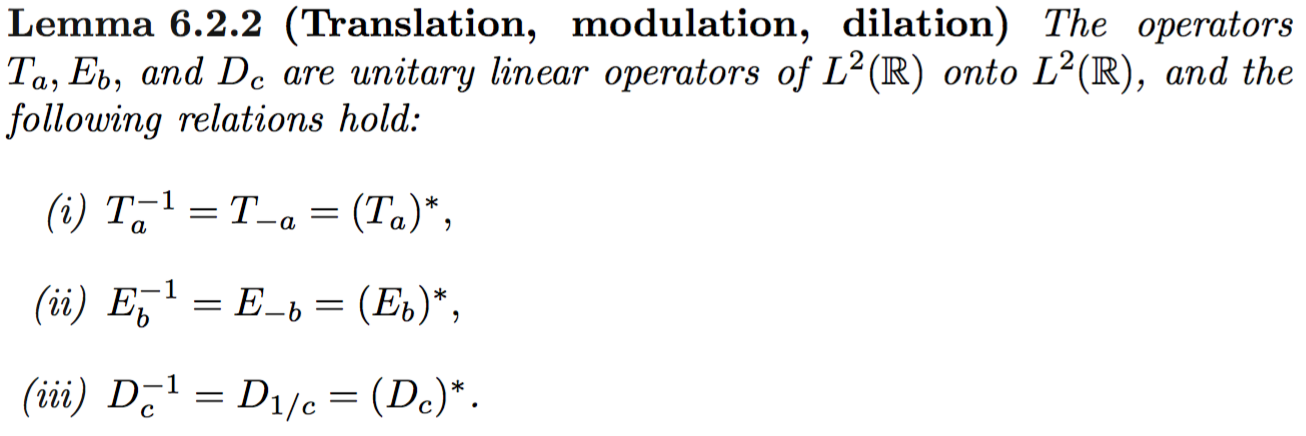
\includegraphics[width=0.9\textwidth]{fig/lemma622}
\end{figure}

\subsection*{Solution:}
In order to say anything about the adjoint operator, we must first see if it is well defined, linear and bounded. 

The dilation operator, as defined in \textbf{definition 6.2.1}, is given as

\begin{gather*}
    (D_c f)(x):= \frac{1}{\sqrt{c}}f(\frac{x}{c}), \: \: x \in \mathbb{R},\: c \: > \: 0.
\end{gather*}

If we assume a function $f(x) \in L^2(\mathbb{R})$, is $(D_c f)(x)$ then also in $L^2(\mathbb{R})$?

\begin{gather*}
    \int_{-\infty}^{\infty} |D_c f(x)|^2 \text{d}x = \int_{-\infty}^{\infty} \left|\frac{1}{\sqrt{c}}f(\frac{x}{c})\right|^2 \text{d}x = \\
    \int_{-\infty}^{\infty} \left|\frac{1}{\sqrt{c}}f(u)\right|^2 c\:\text{d}u = 
    \frac{c}{\sqrt{c}^2}\int_{-\infty}^{\infty} \left|f(u)\right|^2 \text{d}u = \\
    \int_{-\infty}^{\infty} \left|f(u)\right|^2 \text{d}u < \infty
\end{gather*}
$(D_c f)(x) \in L^2(\mathbb{R})$, so $D_c$ is well defined. Now we check for linearity using \textbf{eq. (2.6) section 2.4}

\begin{gather*}
    D_c(\alpha f + \beta g)(x) = \frac{1}{\sqrt{c}}(\alpha f + \beta g)(\frac{x}{c}) = \\
    \alpha \frac{1}{\sqrt{c}} f (\frac{x}{c})+ \beta \frac{1}{\sqrt{c}} g (\frac{x}{c}) = \alpha D_c f(x) + \beta D_c g(x) 
\end{gather*}
The operator is linear. For the bounded criteria we use \textbf{definition 2.4.1} and the result from being well defined

\begin{gather*}
    \int_{-\infty}^{\infty} |D_c f(x)|^2 \text{d}x = || D_cf||_2^2 = \int_{-\infty}^{\infty} \left|f(u)\right|^2 \text{d}u = ||f||_2^2 \Rightarrow \\
    ||D_cf||_2 = ||f||_2
\end{gather*}
So the operator is bounded on $L^2(\mathbb{R})$ with the norm of the operator $||T|| = 1$. 

Now we can look at the adjoint operator as defined in \textbf{section 4.5}, using the inner product. 

\begin{gather*}
    \langle D_cf , g \rangle = \int_{-\infty}^{\infty} \frac{1}{\sqrt{c}}f(\frac{x}{c})\: \overline{g(x)} \text{d}x = \\
    \int_{-\infty}^{\infty} \frac{1}{\sqrt{c}}f(u)\: \overline{g(u c)} c \text{d}x = \int_{-\infty}^{\infty} f(u)\: \overline{ \sqrt{c} \;g(u c)} \text{d}x = \\
    \langle f, D_{1/c} g \rangle
\end{gather*}

We also know from the definition of the adjoint operator, that $\langle D_cf, g \rangle = \langle f, D_c^* g \rangle$, so from \textbf{lemma 4.4.2} we have that $D_{1/c} g =D_c^* g$ leaving us with $D_{1/c}$ and $D_c^*$ as the same operator. So is this a unitary operator?

\begin{gather*}
    D_c D_c^* = D_c D_{1/c}  = I
\end{gather*}
and
\begin{gather*}
     D_c^*D_c = D_{1/c}D_c   = I
\end{gather*}
    By definition, the operator $D_c$ is unitary. 
    
    
    
\begin{figure}[H]
    \centering
    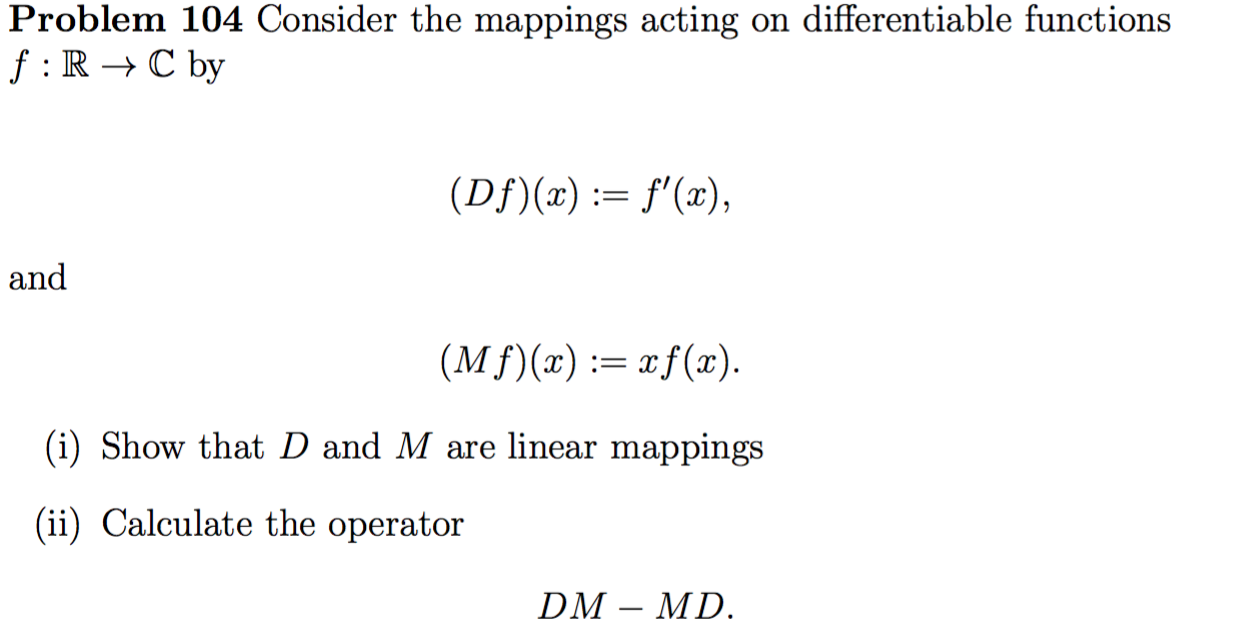
\includegraphics[width=\textwidth]{fig/opg104}
\end{figure}

\subsection*{Solution (i):}
Since we are mapping from $\mathbb{R}$ into $\mathbb{C}$, we assume the operators to be well defined, since we have no restrictions of being normalisable or continuity. Looking at linearity we get

\begin{gather*}
    D(\alpha f + \beta g)(x) = (\alpha f + \beta g)'(x) = \\
    \alpha f'(x) + \beta g'(x) =  \alpha Df(x) + \beta Dg(x) 
\end{gather*}
$D$ is linear.

\begin{gather*}
    M(\alpha f + \beta g)(x) = x(\alpha f + \beta g)(x) =\\
    \alpha xf (x) + \beta xg(x) = \alpha Mf (x) + \beta Mg(x)
\end{gather*}
$M$ is linear.

\subsection*{Solution (ii):}
Calculating the commutator $[D,M]$ we keep in mind, that operators only make sense when applied to a function, therefore we introduce a dummy-function $f(x)$ which they can act upon (the dummy-function will be remove afterwards). 

\begin{gather*}
    [D,M]f(x) = D(Mf(x)) - M(Df(x)) = \\
    \frac{d}{dx}(xf(x)) - x\frac{d}{dx}(f(x)) = \\ f(x)+xf'(x)-xf'(x) = f(x)
\end{gather*}
Dividing by the dummy-function we get $[D,M] = 1$.

\begin{figure}[H]
    \centering
    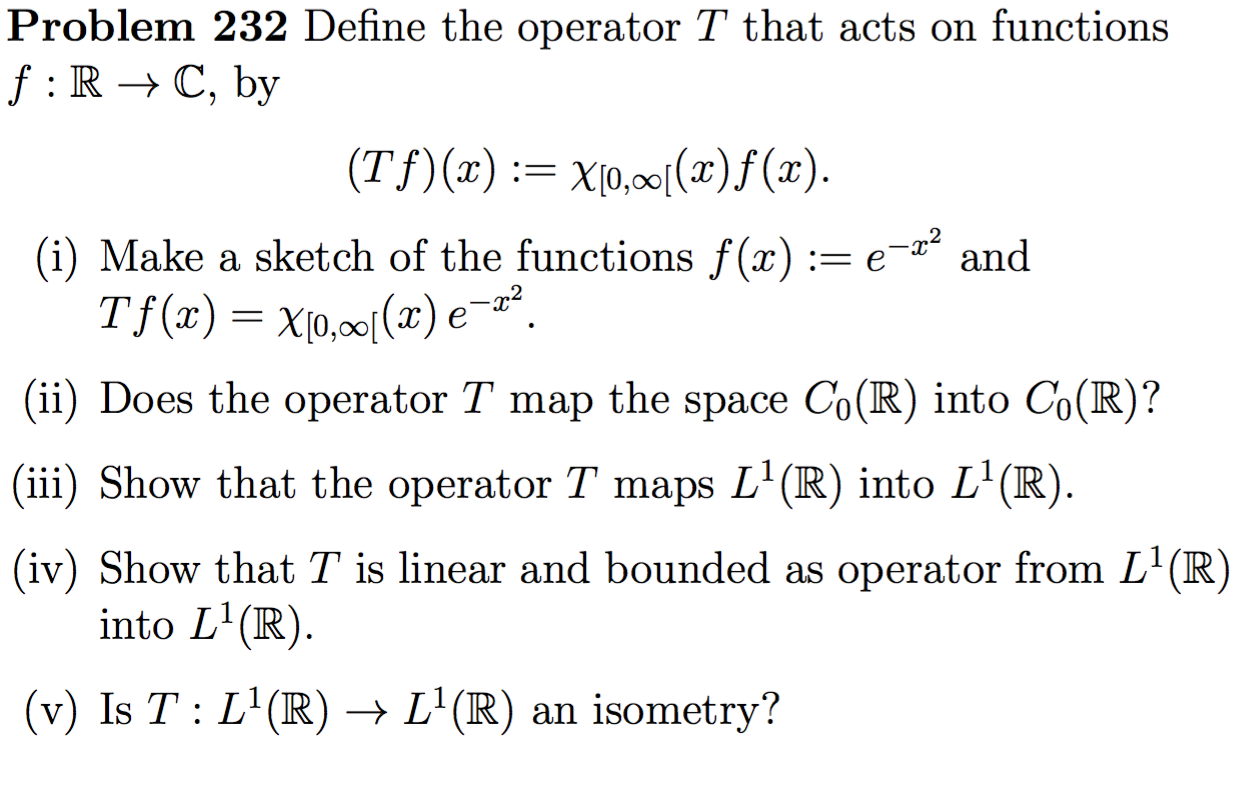
\includegraphics[width=\textwidth]{fig/opg232}
\end{figure}

\subsection*{Solution (i):}
Sketches of $f(x)$ and $Tf(x)$
\begin{figure}[H]
\centering
    \begin{subfigure}{0.495\textwidth}
    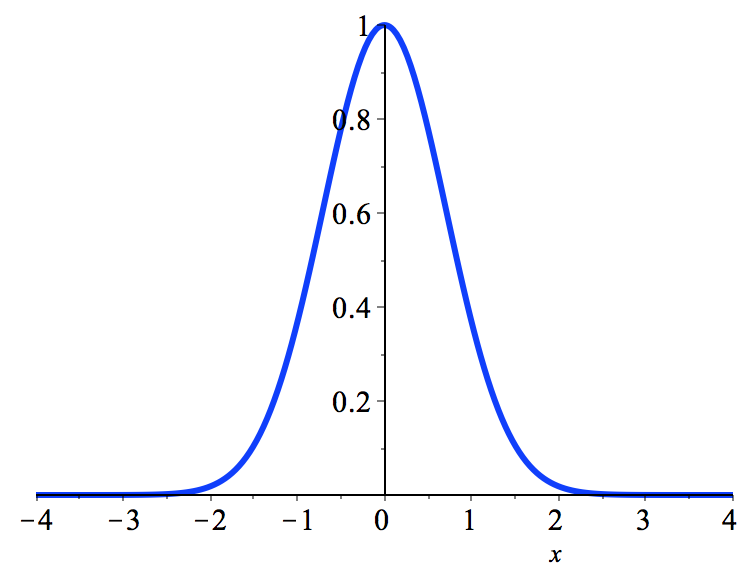
\includegraphics[width=0.9\linewidth, height=4cm]{fig/sketch1}
    \caption*{$f(x)=\text{exp}(-x^2)$}
    \end{subfigure}
    \begin{subfigure}{0.495\textwidth}
    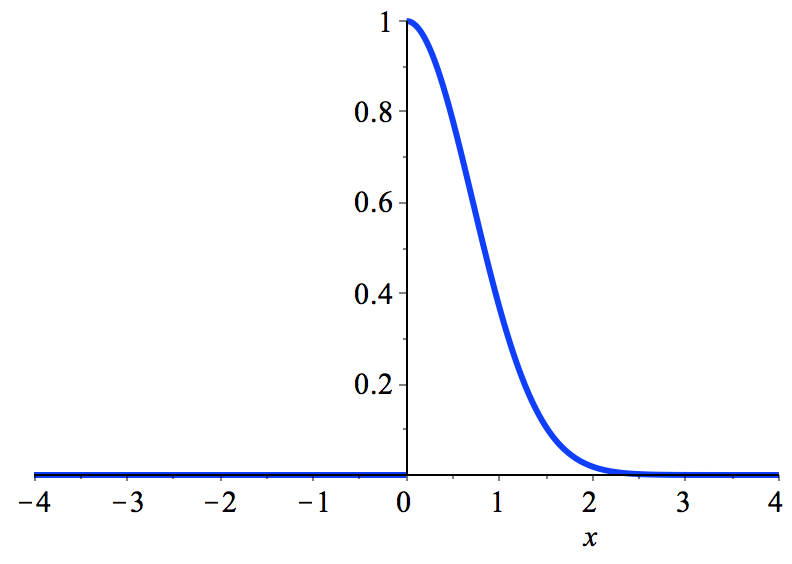
\includegraphics[width=0.9\linewidth, height=4cm]{fig/sketch2}
    \caption*{$Tf(x)=\chi_{[0,\infty[}\text{exp}(-x^2)$}
    \end{subfigure}
\end{figure}


\subsection*{Solution (ii):}

No, $Tf(x) \notin C_0(\mathbb{R}) \: \forall \: f \in C_0(\mathbb{R})$ as it not necessarily is continuous.

\subsection*{Solution (iii):}
$T:L^1(\mathbb{R}) \rightarrow L^1(\mathbb{R})$ : 

\begin{gather*}
    \int_{-\infty}^{\infty} |f(x)| \text{d}x = \int_{-\infty}^{0} |f(x)| \text{d}x + \int_{0}^{\infty} |f(x)| \text{d}x \geq \\
    \int_{0}^{\infty} |f(x)| \text{d}x = \int_{-\infty}^{\infty} |\chi_{[0,\infty[}(x)f(x)| \text{d}x \Rightarrow \\
    \int_{-\infty}^{\infty} |Tf(x)| \text{d}x \leq  \int_{-\infty}^{\infty} |f(x)| \text{d}x < \infty
\end{gather*}

So the operator maps from $L^1(\mathbb{R})$ into $L^1(\mathbb{R})$.

\subsection*{Solution (iv):}
Since we know that the operator is well defined on $L^1(\mathbb{R})$, we can check if it is linear and bounded (the same procedure as in previous problems).

\begin{gather*}
    T(\alpha f + \beta g)(x) = \chi_{[0,\infty[}(x)(\alpha f + \beta g)(x) =\\
    \alpha\chi_{[0,\infty[}(x) f (x)+ \beta \chi_{[0,\infty[}(x) g(x) = \alpha Tf(x) + \beta Tg(x)
\end{gather*}
The operator is linear. When checking if the operator is bounded, we use the result from (iii)

\begin{gather*}
    \int_{-\infty}^{\infty} |Tf(x)| \text{d}x = ||Tf||_1 \leq \int_{-\infty}^{\infty} |f(x)| \text{d}x = ||f||_1 \Rightarrow \\
    ||Tf||_1 \leq K||f||_1
\end{gather*}
With $K=1$. The operator is bounded on $L^1(\mathbb{R})$.  

\subsection*{Solution(v):}
If the operator was an isometry, using definition 2.4.5, the norm $||Tf||_1$ must equal $||f||_1$, which is only the case if the integral in the calculations from (iii) is zero:

\begin{gather*}
    \int_{-\infty}^{\infty} |f(x)| \text{d}x = \int_{-\infty}^{0} |f(x)| \text{d}x + \int_{0}^{\infty} |f(x)| \text{d}x \Rightarrow \\
    ||f||_1 = \int_{-\infty}^{0} |f(x)| \text{d}x + ||Tf||_1 \neq ||Tf||_1 \: \forall f \in L^1(\mathbb{R})
\end{gather*}

The operator is not an isometry in $L^1(\mathbb{R})$.

\end{document}